\documentclass[../main.tex]{subfiles}
\graphicspath{ {../img/} }


\begin{document}


	\chapter{Our implementation and design}


    \section{Thigs necessary for the project we had to either find or makes.}

    Our project had different parts.

    \begin{itemize}

        \item Make a sandboxing environment, to test it, while been sure that it can't escape. 
        We used qemu and unshare to make an environnment that couldn't reach the external network.
        In the end, it wasn't really usefull to make it, because we decided that for the demo, the victims ip should be knowed at launched time, so that we won't see unexpected things in the final demo. 

        \item Find an exploit to use. 
        It had to be a remote code execution, easy to setup, and easy to exploit, because it's not in the purpose of the project to find a new vulnerability, make a exploit or another crazy thing like that.
        We spend hours looking for the perfect exploit, and in the end, we find somebody else project on github, that was doing exactly what we were looking for.
        (https://github.com/opsxcq/
        exploit-CVE-2014-6271)
        Thanks to opsxcq works, we had an easy vulnerability to exploit.
        We choosed shellshock, CVE-2014-6271.
        We find in opsxcq repository, a vulnerable docker image to shellshock CVE-2014-6271, and an easy command to exploit it.
        The other two interested vulnerability that we found in his repos, but that in the end we choosed to not use, was CVE-2016-10033 and CVE-2017-7494.
        There were both unadapted to our needs because of how difficults they would makes us write the exploit.
        We also find Log4J, but in the end decided that we would better to abandon it, and try an easier vulnerability to exploit.

        \item Demonstrate the botnet.
        Like all botnet run things, we had to find a way to prove that the botnet has really taken control of several machine.
        For that, we made one more Vm, that we called vulnerableDOS. We simply run wireshark into, and once the botnet has taken control of the bots, it will make them ping our machine.
        At first, we wanted to make our botnet run an actual DDOS attack on the vulnerableDOS machine, but because it's not in the purpose of the project to make it run a complex attack, our goal is just to prove that we have indeed taken control of the vulnerables machines, we choosed to do only ping.

    \end{itemize}

    Obviously, we also had to make the actual botnet.


    \vspace{10pt}

    \section{design explanations about the botnet.}


    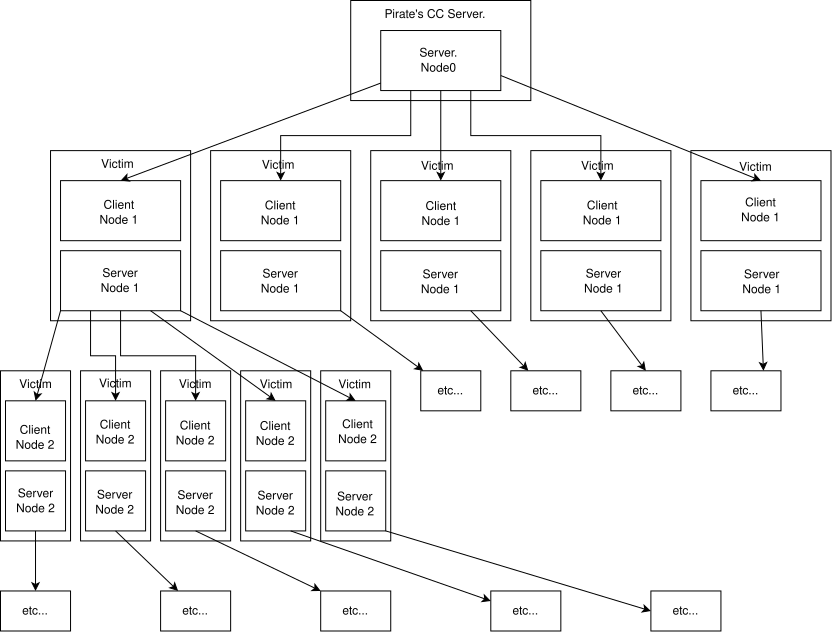
\includegraphics[width=450pt]{botnet.png}




\end{document}
